\documentclass[11pt]{article}
\usepackage[margin=1in]{geometry}
\usepackage{amsmath, amssymb, amsthm}
\usepackage{graphicx}
\usepackage{xcolor}
\usepackage{hyperref}
\usepackage{algorithm}
\usepackage{algpseudocode}
\usepackage{setspace}
\usepackage{biblatex}
\usepackage{arydshln}
\usepackage{subcaption}
\usepackage{mathtools}
\setstretch{1.15}
\addbibresource{references.bib} %Import the bibliography file

\title{\textbf{paper yoyos quasi-static model}}
\author{Brandon Wong, Ben Foster}
\date{\today}

\begin{document}

\maketitle


\section{Geometric model}\label{sec:setup}
\begin{figure}
    \centering
    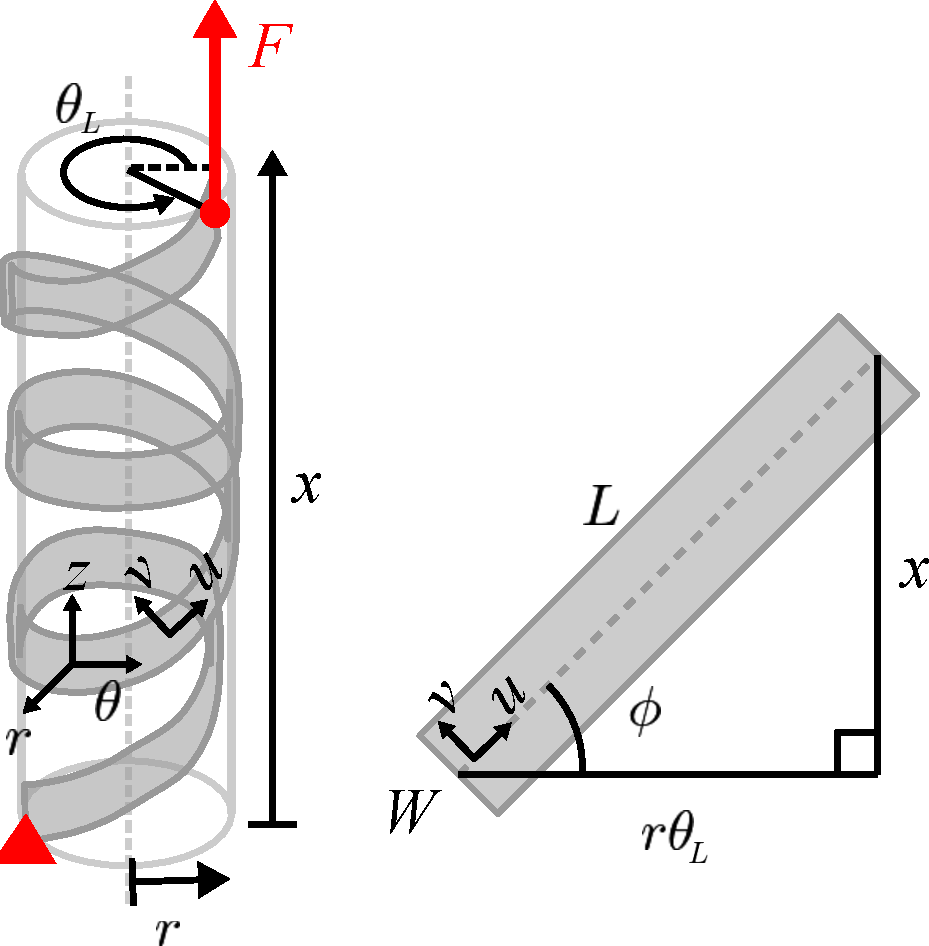
\includegraphics[width=0.5\textwidth]{figs/capstan_helix.pdf}
    \caption{in progress}\label{fig:setup}
\end{figure}

The system can be modelled as a constant-width rectangular ribbon of negligible thickness wrapped around a uniform-radius cylinder at a uniform pitch. One end of the ribbon is fixed in place to prevent rigid body motion, while the other (``active'' end) is displaced in the $z$ direction (the axis of the cylinder). Refer to Figure~\ref{fig:setup} for a visual representation of the system. The system has the following geometric constants:
\begin{itemize}
    \item $L$: the length of the unrolled rectangle.
    \item $W$: the width of the unrolled rectangle. Assume $L \gg W$.
    \item $\theta_L$: the total wind angle of the helix, which is fixed based on the boundary conditions (the two ends of the ribbon cannot rotate about the $z$-axis relative to one another, only translate along it, so the total number of turns is a fixed topological property of how the ribbon was wound and does not change as it is pulled). $\theta_L = 2\pi n$ where $n$ is the number of winds around the $z$ axis (not necessarily integer).
\end{itemize}

The state of the system is parametrized by the parameter $x$, which describes how far the active end has displaced in the $z$ direction relative to the base end.

\subsection{Coordinate systems}
Positions on the helix can be described with local surface $u,v$ coordinates, which describe the unrolled rectangle. The $u$ direction runs along the length of the unrolled rectangle, and the $v$ direction runs across its width. Alternatively, positions can be described in 3d space using cylindrical $r,\theta,z$ coordinates.

To simplify the geometry, we assume that the helix has a constant radius $r$ and a constant pitch angle $\phi$ (the angle the local $\hat{u}$ makes with the $r,\theta$ plane). Equivalently, the local orthonormal frame $(\hat u,\hat v)$ tangent to the ribbon surface is related to the cylinder's own natural frame $(\hat\theta,\hat z)$ by a rotation through the angle $\phi$:
\begin{equation}\label{eq:frame_rotation}
    \hat u = \cos\phi\,\hat\theta + \sin\phi\,\hat z, \qquad
    \hat v = -\sin\phi\,\hat\theta + \cos\phi\,\hat z.
\end{equation}

We now use Eq.~\eqref{eq:frame_rotation} to relate the geometric constants $L,\theta_L$ to the pitch angle $\phi$ and radius $r$ at a given extension $x$. From Eq.~\eqref{eq:frame_rotation}, $\hat u$ has $z$-component $\sin\phi$, so moving a distance $\mathrm du$ along the ribbon's own length produces an axial displacement $\mathrm dz=\sin\phi\,\mathrm du$. Since $\phi$ is constant along the whole ribbon at a given (frozen) extension $x$, integrating this from the base end ($u=0$) to the active end ($u=L$) gives a total axial displacement of $L\sin\phi$. By definition, this total axial displacement between the two ends of the ribbon is exactly $x$, so
\begin{equation}\label{eq:phi}
    x = L\sin\phi \qquad\Longrightarrow\qquad \phi = \sin^{-1}\left(\frac{x}{L}\right).
\end{equation}
Likewise, $\hat u$ has $\theta$-component $\cos\phi$, so moving a distance $\mathrm du$ along the ribbon produces a circumferential arc length $r\,\mathrm d\theta = \cos\phi\,\mathrm du$. Integrating over the whole ribbon length $L$, the ribbon sweeps out a total circumferential arc length $L\cos\phi$. This total arc length must also equal $r\theta_L$ (arc length equals radius times swept angle), since by construction the ribbon winds through the fixed total angle $\theta_L$ regardless of $x$. Equating the two expressions for this arc length and using $\cos\phi=\sqrt{1-\sin^2\phi}$ together with Eq.~\eqref{eq:phi} gives
\begin{equation}\label{eq:r}
    r\theta_L = L\cos\phi \qquad\Longrightarrow\qquad r = \frac{L}{\theta_L}\cos\phi = \frac{L}{\theta_L}\sqrt{1-\frac{x^2}{L^2}} = \frac{\sqrt{L^2 - x^2}}{\theta_L}.
\end{equation}

\subsection{Position vector}\label{sec:position}
An area element $du \times dv$ at point $(u,v)$ has a position vector given in cylindrical coordinates. We build this up from Eq.~\eqref{eq:frame_rotation}: since $\hat u = \cos\phi\,\hat\theta+\sin\phi\,\hat z$, moving along the ribbon by $\mathrm du$ produces $r\,\mathrm d\theta = \cos\phi\,\mathrm du$ and $\mathrm dz = \sin\phi\,\mathrm du$; since $\hat v = -\sin\phi\,\hat\theta + \cos\phi\,\hat z$, moving across the width by $\mathrm dv$ produces $r\,\mathrm d\theta = -\sin\phi\,\mathrm dv$ and $\mathrm dz=\cos\phi\,\mathrm dv$. Integrating these (at fixed, frozen $x$, so $r$ and $\phi$ are constants) from the reference point $(u,v)=(0,0)$ gives
\begin{equation}\label{eq:position}
    \vec{p}(u,v,x) =
    \begin{bmatrix}
        r\\
        \theta\\
        z
    \end{bmatrix} =
    \begin{bmatrix}
        \frac{\sqrt{L^2-x^2}}{\theta_L}\\
        \frac{u \cos\phi - v \sin\phi}{r}\\
        u \sin\phi + v \cos\phi
    \end{bmatrix}.
\end{equation}

\subsection{Local curvature}\label{sec:local_curvature}
A cylinder of radius $r$ has two principal curvatures: $\kappa_\theta = 1/r$ in the circumferential ($\hat\theta$) direction in which it is rolled, and $\kappa_z = 0$ in the axial ($\hat z$) direction in which it is completely flat. Equivalently, the standard cylindrical basis vectors rotate with $\theta$ at the rates
\begin{equation}\label{eq:cyl_basis_deriv}
    \frac{\partial\hat r}{\partial\theta} = \hat\theta, \qquad
    \frac{\partial\hat\theta}{\partial\theta} = -\hat r, \qquad
    \frac{\partial\hat z}{\partial\theta} = 0,
\end{equation}
(the first two follow from writing $\hat r=\cos\theta\,\hat x+\sin\theta\,\hat y$ and $\hat\theta=-\sin\theta\,\hat x+\cos\theta\,\hat y$ in terms of the fixed Cartesian basis and differentiating; the third holds because $\hat z$ does not depend on $\theta$ at all --- this is exactly the statement $\kappa_z=0$).

To differentiate the ribbon's own frame $(\hat u,\hat v,\hat r)$ with respect to $(u,v)$ we use the chain rule through $\theta$. From $\theta(u,v)=(u\cos\phi-v\sin\phi)/r$ (Eq.~\ref{eq:position}), holding $x$ --- hence $\phi,r$ --- fixed,
\begin{equation}\label{eq:dtheta}
    \frac{\partial\theta}{\partial u} = \frac{\cos\phi}{r}, \qquad \frac{\partial\theta}{\partial v} = -\frac{\sin\phi}{r}.
\end{equation}
Combining Eq.~\eqref{eq:cyl_basis_deriv} and Eq.~\eqref{eq:dtheta} via the chain rule (e.g.\ $\partial\hat r/\partial u = (\partial\hat r/\partial\theta)(\partial\theta/\partial u)$) gives
\begin{equation}\label{eq:cyl_basis_uv}
    \frac{\partial\hat r}{\partial u} = \frac{\cos\phi}{r}\hat\theta, \qquad
    \frac{\partial\hat r}{\partial v} = -\frac{\sin\phi}{r}\hat\theta, \qquad
    \frac{\partial\hat\theta}{\partial u} = -\frac{\cos\phi}{r}\hat r, \qquad
    \frac{\partial\hat\theta}{\partial v} = \frac{\sin\phi}{r}\hat r,
\end{equation}
with $\hat z$ constant in $u,v$ throughout. Now differentiate $\hat u,\hat v$ themselves, using $\hat u=\cos\phi\,\hat\theta+\sin\phi\,\hat z$, $\hat v=-\sin\phi\,\hat\theta+\cos\phi\,\hat z$ (Eq.~\ref{eq:frame_rotation}) with $\phi$ held fixed:
\begin{equation}\label{eq:duv_raw}
    \begin{aligned}
    \frac{\partial\hat u}{\partial u} &= \cos\phi\,\frac{\partial\hat\theta}{\partial u} = -\frac{\cos^2\phi}{r}\hat r, &
    \frac{\partial\hat u}{\partial v} &= \cos\phi\,\frac{\partial\hat\theta}{\partial v} = \frac{\sin\phi\cos\phi}{r}\hat r, \\
    \frac{\partial\hat v}{\partial u} &= -\sin\phi\,\frac{\partial\hat\theta}{\partial u} = \frac{\sin\phi\cos\phi}{r}\hat r, &
    \frac{\partial\hat v}{\partial v} &= -\sin\phi\,\frac{\partial\hat\theta}{\partial v} = -\frac{\sin^2\phi}{r}\hat r.
    \end{aligned}
\end{equation}
The same three coefficients, $\cos^2\phi/r$, $\sin^2\phi/r$, and $\sin\phi\cos\phi/r$ (the last one twice), keep reappearing; we name them for convenience,
\begin{equation}\label{eq:curvatures}
    \kappa_{uu} := \frac{\cos^2\phi}{r}, \qquad
    \kappa_{vv} := \frac{\sin^2\phi}{r}, \qquad
    \kappa_{uv} := \frac{\sin\phi\cos\phi}{r},
\end{equation}
so that Eq.~\eqref{eq:duv_raw} reads $\partial\hat u/\partial u=-\kappa_{uu}\hat r$, $\partial\hat u/\partial v=\kappa_{uv}\hat r$, $\partial\hat v/\partial u=\kappa_{uv}\hat r$, $\partial\hat v/\partial v=-\kappa_{vv}\hat r$.

\paragraph{What $\kappa_{uv}$ means.} $\kappa_{uu}$ and $\kappa_{vv}$ are the ordinary curvatures of the $u$- and $v$-coordinate curves themselves: $\kappa_{uu}$ is how fast $\hat u$ tips toward $\hat r$ per unit distance moved \emph{along} $\hat u$, and likewise $\kappa_{vv}$ for $\hat v$ along $\hat v$. $\kappa_{uv}$ is instead a \emph{cross} rate: how fast $\hat u$ tips toward $\hat r$ per unit distance moved in the $v$-direction --- equivalently, how fast $\hat v$ tips toward $\hat r$ per unit distance moved in the $u$-direction, since Eq.~\eqref{eq:duv_raw} gives the same coefficient for both. It is not a slope like $\mathrm dv/\mathrm du$; it has the same units (one over length) and the same geometric meaning as $\kappa_{uu},\kappa_{vv}$ --- a rate at which a tangent direction tilts toward the surface normal --- just for a mixed pair of directions rather than a single one.

Concretely, $\kappa_{uv}$ arises above because $\hat u,\hat v$ are each a mix of $\hat\theta$ and $\hat z$ (Eq.~\ref{eq:frame_rotation}), and only the $\hat\theta$ part of either vector rotates as $\theta$ changes ($\hat z$ does not, Eq.~\ref{eq:cyl_basis_deriv}). Moving in $v$ changes $\theta$ (Eq.~\ref{eq:dtheta}), and therefore rotates the $\hat\theta$-component of $\hat u$ toward $\hat r$ even though $v$ is not $\hat u$'s own direction --- that leftover rotation is exactly $\kappa_{uv}$. Put differently: $\hat u,\hat v$ are rotated by $\phi$ away from the cylinder's own principal directions $\hat\theta,\hat z$, which have no such cross term ($\hat\theta$ only ever rotates toward $\hat r$ as $\theta$ itself changes, never as $z$ changes, and $\hat z$ never rotates at all); $\kappa_{uv}$ is exactly the off-diagonal curvature this rotation introduces. Consistent with this, $\kappa_{uv}=\sin\phi\cos\phi/r$ vanishes at $\phi=0,90^\circ$ (where $\hat u,\hat v$ realign with $\hat\theta,\hat z$) and is largest at $\phi=45^\circ$.

\paragraph{Rotation of $\hat r$.} It remains to differentiate $\hat r$ itself. We already have $\partial\hat r/\partial u,\partial\hat r/\partial v$ in terms of $\hat\theta$ (Eq.~\ref{eq:cyl_basis_uv}); to express them in terms of $\hat u,\hat v$ instead, invert Eq.~\eqref{eq:frame_rotation} for $\hat\theta$ (solving its two equations for $\hat\theta,\hat z$ in terms of $\hat u,\hat v$ gives $\hat\theta=\cos\phi\,\hat u-\sin\phi\,\hat v$). Substituting,
\begin{equation}
    \frac{\partial\hat r}{\partial u} = \frac{\cos\phi}{r}\hat\theta = \frac{\cos\phi}{r}\big(\cos\phi\,\hat u-\sin\phi\,\hat v\big) = \kappa_{uu}\hat u-\kappa_{uv}\hat v,
\end{equation}
and the identical substitution into $\partial\hat r/\partial v=-\frac{\sin\phi}{r}\hat\theta$ gives $\partial\hat r/\partial v=-\kappa_{uv}\hat u+\kappa_{vv}\hat v$. Collecting everything derived in this section,
\begin{equation}\label{eq:frame_rotation_rates}
    \begin{aligned}
    \frac{\partial\hat r}{\partial u} &= \kappa_{uu}\hat u - \kappa_{uv}\hat v, &
    \frac{\partial\hat r}{\partial v} &= -\kappa_{uv}\hat u + \kappa_{vv}\hat v, \\
    \frac{\partial\hat u}{\partial u} &= -\kappa_{uu}\hat r, &
    \frac{\partial\hat u}{\partial v} &= \kappa_{uv}\hat r, \\
    \frac{\partial\hat v}{\partial u} &= \kappa_{uv}\hat r, &
    \frac{\partial\hat v}{\partial v} &= -\kappa_{vv}\hat r.
    \end{aligned}
\end{equation}
Two features of Eq.~\eqref{eq:frame_rotation_rates} are worth flagging because they are used repeatedly below: (i) $\hat u,\hat v$ never rotate into each other ($\partial\hat u/\partial u$ and $\partial\hat u/\partial v$ have no $\hat v$-component, and vice versa) --- this holds because the $u$- and $v$-coordinate lines are straight lines on the flat unrolled rectangle, hence remain geodesics after the isometric wrapping into a helix, and a curve's own tangent frame only rotates toward the surface normal along a geodesic, never within the tangent plane; (ii) the rotation matrix is antisymmetric, e.g.\ $\partial\hat u/\partial u\cdot\hat r=-\partial\hat r/\partial u\cdot\hat u$, as required for any rotating orthonormal frame.


\section{Stress balance}\label{sec:equilibrium}
We will model the paper yoyo as a thin shell of small but finite thickness $t\ll r$. Because the ribbon's thickness ultimately carries the boundary tractions responsible for friction (Section~\ref{sec:friction}), we work throughout with its full three-dimensional stress state. We use $\zeta\in\left[-\frac{t}{2},\frac{t}{2}\right]$ for the coordinate measuring position through the thickness, i.e., displacement from the mid-surface along $\hat r$: a general material point is at $\vec p(u,v,x)+\zeta\hat r(u,v)$, with $\vec p(u,v,x)$ the mid-surface position of Eq.~\eqref{eq:position}. At a point $(u,v,\zeta)$ the material carries the full Cauchy stress tensor
\begin{equation}
    \sigma = \begin{pmatrix}\sigma_{uu}&\sigma_{uv}&\sigma_{ur}\\ \sigma_{uv}&\sigma_{vv}&\sigma_{vr}\\ \sigma_{ur}&\sigma_{vr}&\sigma_{rr}\end{pmatrix}.
\end{equation}
There are six independent components: the in-plane stresses $\sigma_{uu},\sigma_{uv},\sigma_{vv}$; the transverse shears $\sigma_{ur},\sigma_{vr}$, by which the ribbon can transmit a load sideways from one part of its width to another; and $\sigma_{rr}$, the normal pressure caused by layer-layer contact at the ribbon's surface.

We perform a force balance on a differential volume element $\mathrm du\times\mathrm dv\times\mathrm d\zeta$. On each of its six faces there is a traction vector: on the $u$-face (outward normal $\hat u$), the traction is $\vec t_u=\sigma_{uu}\hat u+\sigma_{uv}\hat v+\sigma_{ur}\hat r$, and similarly $\vec t_v=\sigma_{uv}\hat u+\sigma_{vv}\hat v+\sigma_{vr}\hat r$ on the $v$-face and $\vec t_\zeta=\sigma_{ur}\hat u+\sigma_{vr}\hat v+\sigma_{rr}\hat r$ on the $\zeta$-face. Because $t\ll r$, the element can be approximated as a rectangular prism, so the net force on the element is
\begin{equation}
    \left(\frac{\partial\vec t_u}{\partial u}+\frac{\partial\vec t_v}{\partial v}+\frac{\partial\vec t_\zeta}{\partial\zeta}\right)\mathrm du\,\mathrm dv\,\mathrm d\zeta = 0.
\end{equation}
However, because $\hat u,\hat v,\hat r$ themselves depend on $u,v$ (Eq.~\ref{eq:frame_rotation_rates}), differentiating $\vec t_u,\vec t_v,\vec t_\zeta$ produces extra terms beyond the plain derivatives of the stress components. For example, expanding $\frac{\partial}{\partial u}(\sigma_{uu}\hat u)$ includes a curvature-weighted term in the $\hat r$ direction,
\begin{equation}
    \frac{\partial}{\partial u} (\sigma_{uu} \hat u) = \frac{\partial \sigma_{uu}}{\partial u}\hat u + \sigma_{uu}\frac{\partial \hat u}{\partial u}
    = \frac{\partial \sigma_{uu}}{\partial u}\hat u - \kappa_{uu}\sigma_{uu}\hat r,
\end{equation}
the additional curvature-weighted terms reflecting the fact that the element is not perfectly planar, so in-plane stresses are slightly rotated to have a small out-of-plane component, and vice versa. Expanding every term this way (using Eq.~\ref{eq:frame_rotation_rates} throughout) and sorting by component gives three scalar force-balance equations, exact to leading order in $\frac{t}{r}$:
\begin{align}
    \hat u:\quad &\boxed{\frac{\partial\sigma_{uu}}{\partial u}+\frac{\partial\sigma_{uv}}{\partial v}+\frac{\partial\sigma_{ur}}{\partial\zeta} + \kappa_{uu}\sigma_{ur} - \kappa_{uv}\sigma_{vr} = 0} \label{eq:inplane_u_full}\\
    \hat v:\quad &\boxed{\frac{\partial\sigma_{uv}}{\partial u}+\frac{\partial\sigma_{vv}}{\partial v}+\frac{\partial\sigma_{vr}}{\partial\zeta} - \kappa_{uv}\sigma_{ur} + \kappa_{vv}\sigma_{vr} = 0} \label{eq:inplane_v_full}\\
    \hat r:\quad &\boxed{\frac{\partial\sigma_{ur}}{\partial u}+\frac{\partial\sigma_{vr}}{\partial v}+\frac{\partial\sigma_{rr}}{\partial\zeta} - \kappa_{uu}\sigma_{uu}+2\kappa_{uv}\sigma_{uv}-\kappa_{vv}\sigma_{vv} = 0} \label{eq:outofplane_r_full}
\end{align}

Equilibrium alone gives three equations for six unknown stress components. Because $t$ is small, however, we make a first-order approximation that each stress component varies linearly through $t$: knowing its two boundary values at $\zeta=\pm\frac{t}{2}$, for every $(u,v)$, is then equivalent to knowing the full through-thickness profile. Section~\ref{sec:friction} supplies exactly those boundary values for $\sigma_{ur},\sigma_{vr},\sigma_{rr}$, from layer-layer contact; Section~\ref{sec:closed_form} carries out the thickness integration itself, retaining --- rather than dropping --- the curvature-weighted terms above.

\begin{figure}
\centering
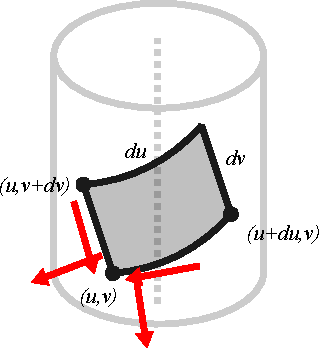
\includegraphics[width=0.5\textwidth]{figs/curved_element.pdf}
\caption{in progress}\label{fig:curved_element}
\end{figure}


\section{Friction}\label{sec:friction}

\subsection{Overlapping neighbors}\label{sec:neighbors}
Because the ribbon is wound around itself, a given area element at $(u,v)$ could physically overlap with another area element one full turn away along the ribbon. Specifically, an area element at point $(u,v)$ overlaps with the neighboring interior layer at point $(u^-,v^-)$ if their cylindrical coordinates have equal $r$ and $z$, but differ by one full turn in $\theta$. We can express this by taking the difference in $\vec{p}$:
\begin{equation}
    \vec{p}(u,v,x) - \vec{p}(u^-,v^-,x) = \begin{bmatrix}
        0\\
        2\pi\\
        0
    \end{bmatrix}.
\end{equation}
Plugging in Eq.~\eqref{eq:position} gives
\begin{align}
    u^- &= u - 2\pi r \cos \phi,\label{eq:uminus}\\
    v^- &= v + 2\pi r \sin \phi.\label{eq:vminus}
\end{align}
By the identical argument with $\theta(u^+,v^+)=\theta(u,v)+2\pi$ (i.e., the neighboring \emph{outer} layer, one full turn further out), the element has an outer overlapping neighbor at
\begin{align}
    u^+ &= u + 2\pi r \cos \phi,\label{eq:uplus}\\
    v^+ &= v - 2\pi r \sin \phi.\label{eq:vplus}
\end{align}
We neglect edge effects where $u^-$ or $u^+$ falls outside the $[0,L]$ bounds --- there is simply no material wound that far, regardless of $v$. Within $[0,L]$, an inner neighbor is present exactly whenever $v^-$ lies within $\left[-\frac{W}{2},\frac{W}{2}\right]$, and an outer neighbor is present exactly whenever $v^+$ lies in $\left[-\frac{W}{2},\frac{W}{2}\right]$, i.e.,
\begin{align}
    \text{Inner neighbor present}&\quad\Longleftrightarrow\quad v\le \frac{W}{2}-2\pi r \sin\phi, \label{eq:overlap_in}\\
    \text{Outer neighbor present}&\quad\Longleftrightarrow\quad v\ge -\frac{W}{2}+2\pi r \sin\phi. \label{eq:overlap_out}
\end{align}

\subsection{Friction direction}\label{sec:slip_direction}
The position vector $\vec p(u,v,x)$ of a material point $(u,v)$ is given by Eq.~\eqref{eq:position}. Substituting Eq.~\eqref{eq:phi} and Eq.~\eqref{eq:r} to expose the dependence on $x$ gives
\begin{equation}
    \vec{p}(u,v,x) =
    \begin{bmatrix}
        \frac{\sqrt{L^2 -x^2 }}{\theta_L }\\
        \frac{u\theta_L}{L}-\frac{v\,x\,\theta_L}{L\sqrt{L^2 -x^2 }}\\
        \frac{ux}{L}+\frac{v\sqrt{L^2 -x^2 }}{L}
    \end{bmatrix}.
\end{equation}
The velocity of a given material point $(u,v)$ as the active end of the ribbon is displaced (i.e., as $x$ changes) is then obtained by taking the partial derivative of each component with respect to $x$:
\begin{equation}\label{eq:velocity}
    \frac{\partial}{\partial x} \vec{p}(u,v,x) =
    \begin{bmatrix}
        \frac{\partial r}{\partial x}\\
        \frac{\partial \theta}{\partial x}\\
        \frac{\partial z}{\partial x}
    \end{bmatrix}=
    \begin{bmatrix}
        -\frac{x}{\theta_L \,\sqrt{L^2 -x^2 }}\\
        -\frac{L\,\theta_L\,v}{{\left(L^2-x^2\right)}^{3/2}}\\
        \frac{u}{L}-\frac{vx}{L\sqrt{L^2 -x^2 }}\\
    \end{bmatrix}.
\end{equation}

We can then plug $u^-,v^-$ into Eq.~\eqref{eq:velocity} to compute the velocity of the element relative to its inner overlapping neighbor, which gives the relative slip direction in the $r,\theta,z$ frame:
\begin{equation}
    \frac{\partial \vec{p}(u,v,x)}{\partial x} - \frac{\partial \vec{p}(u^-,v^-,x)}{\partial x} =
    \begin{bmatrix}
        0\\
        \frac{2\pi\,x}{L^2-x^2}\\
        \frac{2\pi}{\theta_L}
    \end{bmatrix}.
\end{equation}
As expected, there is no relative velocity in the radial direction (i.e., the layers are not lifting away from each other). We can now compute the relative slip direction in the local frame by projecting this slip velocity from the $\theta,z$ basis onto the $u,v$ basis using the relation described by Eq.~\eqref{eq:frame_rotation}. Since $\partial\theta/\partial x$ above is an \emph{angular} rate, we first convert it to a linear (arc-length) rate by multiplying by $r$, giving $v_\theta = r\,\partial\theta/\partial x$; then projecting as just described:
\begin{equation}\label{eq:vslip_raw}
    \vec{v}_{slip}(u,v,x) = \begin{bmatrix}
        \cos\phi & \sin\phi \\
        -\sin\phi & \cos\phi
    \end{bmatrix}
    \begin{bmatrix}
        r\cdot\frac{2\pi\,x}{L^2-x^2}\\
        \frac{2\pi}{\theta_L}
    \end{bmatrix}.
\end{equation}
We simplify this expression by substituting $x$ and $r$ in terms of $\phi$ (Eq.~\eqref{eq:phi},~\eqref{eq:r}) to expose the double-angle combination, then applying double-angle trig identities to factor out common terms. The result is a scaled unit vector:
\begin{equation}
    \vec{v}_{slip}(u,v,x) = \frac{2\pi}{\theta_L\cos\phi} \begin{bmatrix} \sin(2\phi) \\ \cos(2\phi) \end{bmatrix}.
\end{equation}
The prefactor is strictly positive for all $x \in (0,L)$. Therefore, the relative slip velocity points in the direction of the unit vector $(\sin2\phi,\cos2\phi)$ in the local $u,v$ frame, so the Coulomb friction force opposing this motion must point in the opposite direction:
\begin{equation}\label{eq:friction_direction}
    \hat{f} = -\begin{bmatrix} \sin(2\phi) \\ \cos(2\phi) \end{bmatrix}.
\end{equation}

\subsection{Friction magnitude}\label{sec:friction_magnitude}
Let us take a moment to introduce some shorthand notation for the two boundary values of $\sigma_{rr}$ and their sum and difference, which will recur constantly from here on:
\begin{align}
    \sigma_{rr}^\pm &:= \sigma_{rr}\left(\zeta=\pm\frac{t}{2}\right),\\
    \Delta\sigma_{rr} &:= \sigma_{rr}^+-\sigma_{rr}^-,\\
    S_{rr} &:= \sigma_{rr}^++\sigma_{rr}^-.
\end{align}

Recall that Eq.~\eqref{eq:friction_direction} is the friction exerted on the element by the inner layer, which resists the element from sliding forward with $x$. The components of this friction force are equivalent to the shear stresses acting on the inner ($-\hat r$) face. Additionally, the magnitude of the Coulomb friction force is equivalent to the normal pressure $-\sigma_{rr}$ times a friction coefficient $\mu$. By saying this, we assume $\sigma_{rr}\le0$ (the element is under compression), deferring a rigorous justification to Section~\ref{sec:sign_monotonicity}. Therefore,
\begin{align}
    \sigma_{ur}\left(\zeta = -\frac{t}{2}\right) &= -\mu \sigma_{rr}^-\sin(2\phi), \label{eq:sigma_ur_inner}\\
    \sigma_{vr}\left(\zeta = -\frac{t}{2}\right) &= -\mu \sigma_{rr}^-\cos(2\phi). \label{eq:sigma_vr_inner}
\end{align}
By the same argument, the friction exerted by the outer layer is the exact opposite, dragging the element forward, giving the corresponding relationship on the outer ($+\hat r$) face (the sign does not flip, due to the sign convention for shear stresses on opposite faces of an element):
\begin{align}
    \sigma_{ur}\left(\zeta = \frac{t}{2}\right) &= -\mu \sigma_{rr}^+\sin(2\phi), \label{eq:sigma_ur_outer}\\
    \sigma_{vr}\left(\zeta = \frac{t}{2}\right) &= -\mu \sigma_{rr}^+\cos(2\phi). \label{eq:sigma_vr_outer}
\end{align}
Each pair holds only where the corresponding neighbor is actually present (Eq.~\ref{eq:overlap_in}--\ref{eq:overlap_out}); where the neighbor is absent, both shear components vanish along with the contact pressure that would otherwise drive them.

Let thickness-averaged stress components be denoted by a bar, i.e., $\bar\sigma_{ij}:=\frac1t\int_{-\frac t2}^{\frac t2}\sigma_{ij}\,\mathrm d\zeta$. For simplicity, we assume the thickness is small enough that the variation of all stress components through the thickness can be approximated as linear --- so that, for any component, knowing its two boundary values at $\zeta=\pm\frac{t}{2}$ is equivalent to knowing its thickness average (the linear part of the profile drops out of the average). Using Eqs.~\eqref{eq:sigma_ur_inner}--\eqref{eq:sigma_vr_outer}, the thickness-averaged transverse shears come out proportional to $S_{rr}$, not $\Delta\sigma_{rr}$ --- the average of a linear profile is set by the two boundary values \emph{added}, not subtracted:
\begin{align}
    \Aboxed{\bar\sigma_{ur} &= -\frac{\mu}{2}S_{rr}\sin(2\phi)}\label{eq:bar_sigma_ur}\\
    \Aboxed{\bar\sigma_{vr} &= -\frac{\mu}{2}S_{rr}\cos(2\phi)}\label{eq:bar_sigma_vr}
\end{align}

\subsection{Layer-layer contact relationship}\label{sec:layer_layer_contact}
By Newton's third law, two surfaces in contact should experience equal and opposite traction forces. Because the surface normals are opposite, this means they should have equal stresses. It suffices to equate the normal pressures $\sigma_{rr}$ because the transverse shear stresses are related above. Therefore, we get the following recursive relationships to define the boundary stresses, using piecewise gates based on layer contact boundaries:
\begin{align}
    \text{Outer surface:}&\quad \sigma_{rr}^+\left(u,v\right) = \begin{cases}
        \sigma_{rr}^-\left(u^+,v^+\right) & \quad v \ge -\frac{W}{2}+2\pi r \sin\phi\\
        0 &\quad \text{otherwise}
    \end{cases}\label{eq:contact_outer}\\
    \text{Inner surface:}&\quad\sigma_{rr}^-\left(u,v\right) = \begin{cases}
        \sigma_{rr}^+\left(u^-,v^-\right) & \quad v \le \frac{W}{2}-2\pi r \sin\phi\\
        0 &\quad \text{otherwise}
    \end{cases}\label{eq:contact_inner}
\end{align}
Equations~\eqref{eq:contact_outer}--\eqref{eq:contact_inner} recursively relate the boundary stress of one layer to that of its neighbor, one full turn away; propagated far enough in $u$, they reach the outermost wound layer at $u=L$, past which no material is wound at all, so $\sigma_{rr}^+(L,v)=0$ for all $v$ --- the base case that starts the recursion.

We can approximate this recursive relationship with a first-order Taylor expansion. We can also rewrite the piecewise cases using Heaviside step functions $H(x)$, defined by $H(x)=1$ for $x\ge0$ and $H(x)=0$ for $x<0$. Let $H^+:=H\!\left(v+\frac W2-2\pi r\sin\phi\right)$ and $H^-:=H\!\left(v-\frac W2+2\pi r\sin\phi\right)$ be the gates that indicate whether an element has an outer or inner neighbor, respectively. The outer layer contact relationship becomes, writing out $\sigma_{rr}^-(u^+,v^+)=\sigma_{rr}^-(u+2\pi r\cos\phi,v-2\pi r\sin\phi)$ and Taylor-expanding in the (fixed, since $r,\phi$ are frozen at extension $x$) shift $(2\pi r\cos\phi,-2\pi r\sin\phi)$:
\begin{equation}\label{eq:contact_outer_taylor}
    \sigma_{rr}^+(u,v) \approx \left[\sigma_{rr}^-(u,v) + 2\pi r\cos\phi\frac{\partial\sigma_{rr}^-}{\partial u} - 2\pi r\sin\phi\frac{\partial\sigma_{rr}^-}{\partial v}\right]H^+.
\end{equation}
By the identical argument on the inner surface relation,
\begin{equation}\label{eq:contact_inner_taylor}
    \sigma_{rr}^-(u,v) \approx \left[\sigma_{rr}^+(u,v) - 2\pi r\cos\phi\frac{\partial\sigma_{rr}^+}{\partial u} + 2\pi r\sin\phi\frac{\partial\sigma_{rr}^+}{\partial v}\right]H^-.
\end{equation}
Subtracting Eq.~\eqref{eq:contact_outer_taylor} from Eq.~\eqref{eq:contact_inner_taylor} gives an expression for $\Delta\sigma_{rr}=\sigma_{rr}^+-\sigma_{rr}^-$. Depending on the values of $H^+,H^-$ (i.e., on $v,r,\phi$), there are four cases:
\begin{align}
    \text{No contact}&\qquad \Delta\sigma_{rr} = 0\\
    \text{Outer contact only}&\qquad \Delta\sigma_{rr} = \sigma_{rr}^- + 2\pi r\cos\phi\frac{\partial\sigma_{rr}^-}{\partial u} - 2\pi r\sin\phi\frac{\partial\sigma_{rr}^-}{\partial v}\\
    \text{Inner contact only}&\qquad \Delta\sigma_{rr} = -\sigma_{rr}^+ + 2\pi r\cos\phi\frac{\partial\sigma_{rr}^+}{\partial u} - 2\pi r\sin\phi\frac{\partial\sigma_{rr}^+}{\partial v}\\
    \text{Both contacts}&\qquad \boxed{\Delta\sigma_{rr} = \pi r\cos\phi\frac{\partial S_{rr}}{\partial u} - \pi r\sin\phi\frac{\partial S_{rr}}{\partial v}}\label{eq:delta_sigma_rr_both}
\end{align}
All four cases are consistent with the ``both contacts'' case, Eq.~\eqref{eq:delta_sigma_rr_both}, as long as the appropriate gates are applied to force $\sigma_{rr}^+$ and $\sigma_{rr}^-$ individually to zero when the corresponding neighbor is absent.


\section{Compatibility}\label{sec:compatibility}
The previous two sections have dealt only with kinematics and forces. Equilibrium constrains forces to balance on every element of material; it says nothing about whether the resulting stress field is actually consistent with a single, continuous displacement of a real, unbroken sheet. A stress field can satisfy Eqs.~\eqref{eq:inplane_u_full}--\eqref{eq:inplane_v_full} perfectly well and still correspond to a deformation that tears the ribbon or folds it through itself. Ruling that out is genuinely new information, on top of equilibrium, geometry, and friction --- and it is this section's whole job, kept deliberately self-contained: nothing here refers to friction, contact, or any of the machinery of Sections~\ref{sec:equilibrium}--\ref{sec:layer_layer_contact}, so that this remains a statement about \emph{any} plane-stress field on this geometry, to be combined with the rest only once we start assembling the closed system in Section~\ref{sec:closed_form}.

Let the thickness-averaged strain components be $\bar\epsilon_{uu},\bar\epsilon_{vv},\bar\epsilon_{uv}$. Because these come from differentiating a single, well-defined displacement field, they cannot be three independent functions; mixed partial derivatives of the (unknown, but assumed to exist) displacement field must commute, which gives the Saint-Venant compatibility condition
\begin{equation}\label{eq:compat_strain}
    \frac{\partial^2\bar\epsilon_{uu}}{\partial v^2}+\frac{\partial^2\bar\epsilon_{vv}}{\partial u^2}-2\frac{\partial^2\bar\epsilon_{uv}}{\partial u\,\partial v}=0.
\end{equation}
Intuitively: this is the statement that the strain field has to be ``integrable'' back into a displacement --- the elastic analogue of asking that a vector field have zero curl before it can be written as a gradient.

Eq.~\eqref{eq:compat_strain} is a condition on \emph{strain}, and our unknowns are \emph{stress}. Hooke's law, for a linear isotropic material under plane stress, is the bridge between the two. Introducing the material's Young's modulus $E$ and Poisson ratio $\nu$, the thickness-averaged Hooke's law reads
\begin{equation}\label{eq:hookes_law}
    \bar\epsilon_{uu}=\frac1E\big(\bar\sigma_{uu}-\nu\bar\sigma_{vv}\big), \qquad
    \bar\epsilon_{vv}=\frac1E\big(\bar\sigma_{vv}-\nu\bar\sigma_{uu}\big), \qquad
    \bar\epsilon_{uv}=\frac{1+\nu}{E}\bar\sigma_{uv}.
\end{equation}
This is the one genuinely new physical assumption in this section --- everything up to here followed from geometry, equilibrium, and Coulomb friction alone; this is the first place the ribbon's actual material stiffness enters.

Substituting Eq.~\eqref{eq:hookes_law} into Eq.~\eqref{eq:compat_strain} and multiplying through by $E$, the modulus cancels out entirely --- compatibility, once written in terms of stress, doesn't care how stiff the material is, only how it distributes strain between directions ($\nu$):
\begin{equation}\label{eq:compat_stress_raw}
    \boxed{
    \frac{\partial^2\bar\sigma_{uu}}{\partial v^2}-\nu\frac{\partial^2\bar\sigma_{vv}}{\partial v^2}+\frac{\partial^2\bar\sigma_{vv}}{\partial u^2}-\nu\frac{\partial^2\bar\sigma_{uu}}{\partial u^2}-2(1+\nu)\frac{\partial^2\bar\sigma_{uv}}{\partial u\,\partial v}=0.}
\end{equation}
This equation, on its own, involves only $\bar\sigma_{uu},\bar\sigma_{uv},\bar\sigma_{vv}$ and the single material constant $\nu$ --- no friction, no contact, no $\sigma_{rr}$. Section~\ref{sec:closed_form} is where it gets folded together with the (friction-sourced) equilibrium equations of Sections~\ref{sec:equilibrium}--\ref{sec:layer_layer_contact} into one governing PDE.


\section{PDE formulation and closed-form solution}\label{sec:closed_form}
We now assemble the pieces above into a closed system for the stress field. Section~\ref{sec:friction} uses Coulomb friction to fix $\sigma_{ur},\sigma_{vr}$ at the two surfaces $\zeta=\pm\frac{t}{2}$ directly in terms of $\sigma_{rr}$ (Eqs.~\ref{eq:sigma_ur_inner}--\ref{eq:sigma_vr_outer}); combined with the linear-through-thickness approximation of Section~\ref{sec:equilibrium}, this eliminates $\sigma_{ur},\sigma_{vr}$ entirely and reduces every remaining unknown to a function of $(u,v)$ alone: $\bar\sigma_{uu},\bar\sigma_{uv},\bar\sigma_{vv}$ for the in-plane stresses, and $\sigma_{rr}^+,\sigma_{rr}^-$ (equivalently $S_{rr},\Delta\sigma_{rr}$) for the two boundary values of the out-of-plane stress, which cannot be thickness-averaged away since they enter the friction law directly.

\paragraph{Counting equations and unknowns.} There are five unknown fields of $(u,v)$: $\bar\sigma_{uu},\bar\sigma_{uv},\bar\sigma_{vv},\sigma_{rr}^+,\sigma_{rr}^-$. It is tempting to count up every equation derived so far and declare the system closed once the totals match, but that overstates what each piece actually buys. The out-of-plane equilibrium equation (Eq.~\ref{eq:outofplane_r_full}, thickness-integrated below) and the contact recursion (Eq.~\ref{eq:delta_sigma_rr_both}) are \emph{both} statements about $\Delta\sigma_{rr}$ in terms of $S_{rr}$'s gradient --- together they are exactly two equations for the two quantities $S_{rr},\Delta\sigma_{rr}$, and once $\bar\sigma_{uu},\bar\sigma_{uv},\bar\sigma_{vv}$ are known, this pair is already self-contained (Section~\ref{sec:outofplane_integration} solves it explicitly). It supplies no additional constraint on $\bar\sigma_{uu},\bar\sigma_{uv},\bar\sigma_{vv}$ beyond feeding them a source term. So the real gap is the one plane-stress elasticity always has: the two thickness-integrated in-plane equations (Section~\ref{sec:inplane_integration}) relate three unknowns, $\bar\sigma_{uu},\bar\sigma_{uv},\bar\sigma_{vv}$, leaving exactly one relation missing among them. Compatibility (Eq.~\ref{eq:compat_stress_raw}) is that missing relation. Properly accounted for, the closed system is: two in-plane equilibrium equations $+$ one compatibility equation, for $\bar\sigma_{uu},\bar\sigma_{uv},\bar\sigma_{vv}$; and, separately, the out-of-plane equilibrium equation $+$ the contact recursion, for $\sigma_{rr}^+,\sigma_{rr}^-$ --- five equations in total for the five unknowns, but arranged as two coupled subsystems (3-for-3 and 2-for-2) rather than five equations all constraining everything at once.

Boundary conditions: the ribbon is traction-free at its long edges, $\bar\sigma_{uv}=\bar\sigma_{vv}=0$ at $v=\pm\frac W2$; there is no outer neighbor at the active end, $\sigma_{rr}^+=0$ at $u=L$ (with $\sigma_{rr}^-,S_{rr},\Delta\sigma_{rr}$ there fixed by this together with the governing equations, not independently); and the resultant of $\bar\sigma_{uu},\bar\sigma_{uv}$ at $u=L$, projected onto the pulling direction, must equal the applied (Instron) force,
\begin{equation}\label{eq:end_load}
    F(x) = W\big[\bar\sigma_{uu}(L)\sin\phi+\bar\sigma_{uv}(L)\cos\phi\big].
\end{equation}

\subsection{In-plane thickness integration}\label{sec:inplane_integration}
We now integrate the three equilibrium equations through the thickness. Beginning with the $\hat u$ direction, Eq.~\eqref{eq:inplane_u_full},
\begin{align}
    \frac1t\int_{-\frac t2}^{\frac t2}\left(\frac{\partial\sigma_{uu}}{\partial u}+\frac{\partial\sigma_{uv}}{\partial v}+\frac{\partial\sigma_{ur}}{\partial\zeta}+\kappa_{uu}\sigma_{ur}-\kappa_{uv}\sigma_{vr}\right)\mathrm d\zeta &= 0\\
    \frac{\partial\bar\sigma_{uu}}{\partial u}+\frac{\partial\bar\sigma_{uv}}{\partial v}+\frac1t\sigma_{ur}\Big|_{-\frac t2}^{\frac t2}+\kappa_{uu}\bar\sigma_{ur}-\kappa_{uv}\bar\sigma_{vr} &= 0
\end{align}
Substituting Eqs.~\eqref{eq:bar_sigma_ur}--\eqref{eq:bar_sigma_vr} for the thickness-averaged shears, and $\sigma_{ur}\big|_{-t/2}^{t/2}=\sigma_{ur}(t/2)-\sigma_{ur}(-t/2)=-\mu\sin(2\phi)\Delta\sigma_{rr}$ from Eqs.~\eqref{eq:sigma_ur_inner},\eqref{eq:sigma_ur_outer}, then simplifying the curvature term with $\kappa_{uu}\sin2\phi-\kappa_{uv}\cos2\phi=\kappa_{uv}$ (Eq.~\ref{eq:curvatures} and double-angle identities),
\begin{equation}\label{eq:inplane_u_integrated}
    \boxed{\frac{\partial\bar\sigma_{uu}}{\partial u} + \frac{\partial\bar\sigma_{uv}}{\partial v} - \frac{\mu \sin(2\phi)\Delta\sigma_{rr}}{t} - \frac{\mu\sin(2\phi)S_{rr}}{4r} = 0}
\end{equation}
Integrating the $\hat v$ direction, Eq.~\eqref{eq:inplane_v_full}, the same way gives
\begin{equation}\label{eq:inplane_v_integrated}
    \boxed{\frac{\partial\bar\sigma_{uv}}{\partial u} + \frac{\partial\bar\sigma_{vv}}{\partial v} - \frac{\mu \cos(2\phi)\Delta \sigma_{rr}}{t} + \frac{\mu\cos(2\phi)S_{rr}}{4r} = 0}
\end{equation}
These are two equations for the three unknowns $\bar\sigma_{uu},\bar\sigma_{uv},\bar\sigma_{vv}$ (given $\Delta\sigma_{rr},S_{rr}$); Section~\ref{sec:beltrami_michell} supplies the third.

\subsection{Out-of-plane thickness integration}\label{sec:outofplane_integration}
Next, we integrate the $\hat r$ direction, Eq.~\eqref{eq:outofplane_r_full}:
\begin{align}
    \frac1t\int_{-\frac t2}^{\frac t2}\left(\frac{\partial\sigma_{ur}}{\partial u}+\frac{\partial\sigma_{vr}}{\partial v}+\frac{\partial\sigma_{rr}}{\partial\zeta}-\kappa_{uu}\sigma_{uu}+2\kappa_{uv}\sigma_{uv}-\kappa_{vv}\sigma_{vv}\right)\mathrm d\zeta &= 0\\
    \frac{\partial\bar\sigma_{ur}}{\partial u}+\frac{\partial\bar\sigma_{vr}}{\partial v}+\frac1t\Delta\sigma_{rr}-\kappa_{uu}\bar\sigma_{uu}+2\kappa_{uv}\bar\sigma_{uv}-\kappa_{vv}\bar\sigma_{vv} &= 0
\end{align}
Substituting Eqs.~\eqref{eq:bar_sigma_ur}--\eqref{eq:bar_sigma_vr} for $\bar\sigma_{ur},\bar\sigma_{vr}$ (using that $\phi$ is constant across the ribbon, so the derivative passes straight through $\sin2\phi,\cos2\phi$),
\begin{equation}\label{eq:outofplane_exact}
    \Delta\sigma_{rr} = t\big[\kappa_{uu}\bar\sigma_{uu}-2\kappa_{uv}\bar\sigma_{uv}+\kappa_{vv}\bar\sigma_{vv}\big] + \frac{t\mu}{2}\left[\sin(2\phi)\frac{\partial S_{rr}}{\partial u}+\cos(2\phi)\frac{\partial S_{rr}}{\partial v}\right].
\end{equation}
This is one equation in the two unknowns $S_{rr},\Delta\sigma_{rr}$; by itself it is not yet closed. Equating it with Eq.~\eqref{eq:delta_sigma_rr_both} (the alternate, geometric expression for $\Delta\sigma_{rr}$ from the recursive contact relationship) gives
\begin{equation}
    \left(\pi r\cos\phi-\frac{t\mu}{2}\sin(2\phi)\right)\frac{\partial S_{rr}}{\partial u} - \left(\pi r\sin\phi+\frac{t\mu}{2}\cos(2\phi)\right)\frac{\partial S_{rr}}{\partial v} = t\big[\kappa_{uu}\bar\sigma_{uu}-2\kappa_{uv}\bar\sigma_{uv}+\kappa_{vv}\bar\sigma_{vv}\big].
\end{equation}
The $t\mu$ corrections to the two coefficients are smaller than the leading $\pi r\cos\phi,\pi r\sin\phi$ terms by a factor of order $t/r$ (an explicit $t$ against an explicit $r$), so at leading order they drop, leaving the closed transport equation for $S_{rr}$ alone:
\begin{equation}\label{eq:S_transport}
    \boxed{\pi r\cos\phi\,\frac{\partial S_{rr}}{\partial u} - \pi r\sin\phi\,\frac{\partial S_{rr}}{\partial v} = t\big[\kappa_{uu}\bar\sigma_{uu}-2\kappa_{uv}\bar\sigma_{uv}+\kappa_{vv}\bar\sigma_{vv}\big].}
\end{equation}
Given $\bar\sigma_{uu},\bar\sigma_{uv},\bar\sigma_{vv}$, Eq.~\eqref{eq:S_transport} determines $S_{rr}$ (a first-order transport equation, solvable along its characteristics using $\sigma_{rr}^+(L,v)=0$), and $\Delta\sigma_{rr}$ then follows algebraically from Eq.~\eqref{eq:outofplane_exact} at the same leading order, $\Delta\sigma_{rr}\approx t[\kappa_{uu}\bar\sigma_{uu}-2\kappa_{uv}\bar\sigma_{uv}+\kappa_{vv}\bar\sigma_{vv}]$. This is the self-contained 2-for-2 subsystem referred to above.

\subsection{Closing compatibility with friction: the Beltrami--Michell equation}\label{sec:beltrami_michell}
Section~\ref{sec:compatibility} derived Eq.~\eqref{eq:compat_stress_raw} without any reference to friction. We now fold the two together --- this is the one place in the whole derivation where compatibility and the friction-sourced equilibrium equations actually meet. Eq.~\eqref{eq:compat_stress_raw} still has a mixed derivative of $\bar\sigma_{uv}$ in it, which we would rather not carry into the final answer. The trick is to notice that Eqs.~\eqref{eq:inplane_u_integrated}--\eqref{eq:inplane_v_integrated} \emph{already} relate $\partial\bar\sigma_{uv}/\partial v$ and $\partial\bar\sigma_{uv}/\partial u$ to the other fields --- differentiating the first with respect to $u$ and the second with respect to $v$, then adding, produces $2\,\partial^2\bar\sigma_{uv}/\partial u\,\partial v$ on one side and nothing but already-known quantities on the other:
\begin{equation}\label{eq:mixed_elim}
    \begin{aligned}
    2\frac{\partial^2\bar\sigma_{uv}}{\partial u\,\partial v} = &-\left(\frac{\partial^2\bar\sigma_{uu}}{\partial u^2}+\frac{\partial^2\bar\sigma_{vv}}{\partial v^2}\right)
    + \frac{\mu}{t}\left[\sin(2\phi)\frac{\partial\Delta\sigma_{rr}}{\partial u}+\cos(2\phi)\frac{\partial\Delta\sigma_{rr}}{\partial v}\right] \\
    &+ \frac{\mu}{4r}\left[\sin(2\phi)\frac{\partial S_{rr}}{\partial u}-\cos(2\phi)\frac{\partial S_{rr}}{\partial v}\right].
    \end{aligned}
\end{equation}
Substituting Eq.~\eqref{eq:mixed_elim} into Eq.~\eqref{eq:compat_stress_raw}, the coefficients of $\partial^2\bar\sigma_{uu}/\partial u^2$ and $\partial^2\bar\sigma_{vv}/\partial v^2$ both collect to $-\nu+(1+\nu)=1$, matching the coefficient $1$ already sitting on $\partial^2\bar\sigma_{uu}/\partial v^2$ and $\partial^2\bar\sigma_{vv}/\partial u^2$ --- so the four second-derivative terms combine into a plain 2D Laplacian of $\bar\sigma_{uu}+\bar\sigma_{vv}$, giving the Beltrami--Michell equation
\begin{equation}\label{eq:beltrami_michell}
    \boxed{\begin{aligned}
    \nabla^2\big(\bar\sigma_{uu}+\bar\sigma_{vv}\big) = (1+\nu)\bigg\{&\frac{\mu}{t}\left[\sin(2\phi)\frac{\partial\Delta\sigma_{rr}}{\partial u}+\cos(2\phi)\frac{\partial\Delta\sigma_{rr}}{\partial v}\right] \\
    &+ \frac{\mu}{4r}\left[\sin(2\phi)\frac{\partial S_{rr}}{\partial u}-\cos(2\phi)\frac{\partial S_{rr}}{\partial v}\right]\bigg\}.
    \end{aligned}}
\end{equation}
Intuitively, this is a Poisson-type equation: the total in-plane stress $\bar\sigma_{uu}+\bar\sigma_{vv}$ can't vary however it likes --- it has to curve in response to how unevenly the friction forcing is distributed, the way a temperature field curves in response to a heat source. Using the leading-order relation $\Delta\sigma_{rr}\approx t[\kappa_{uu}\bar\sigma_{uu}-2\kappa_{uv}\bar\sigma_{uv}+\kappa_{vv}\bar\sigma_{vv}]$ (Section~\ref{sec:outofplane_integration}), the explicit $t$ cancels the $1/t$ in front of the $\Delta\sigma_{rr}$ term, reducing it to ordinary derivatives of $\bar\sigma_{uu},\bar\sigma_{uv},\bar\sigma_{vv}$; the $S_{rr}$ term does not reduce the same way, since $S_{rr}$ solves the separate transport equation, Eq.~\eqref{eq:S_transport}, rather than an algebraic relation. Equations~\eqref{eq:inplane_u_integrated}, \eqref{eq:inplane_v_integrated}, and \eqref{eq:beltrami_michell} are now three equations for the three unknowns $\bar\sigma_{uu},\bar\sigma_{uv},\bar\sigma_{vv}$, closing the gap identified above.

\subsection{PDE solution}\label{sec:pde_solution}
The system is now closed, but Eq.~\eqref{eq:beltrami_michell} is second order in $v$ while Eqs.~\eqref{eq:inplane_u_integrated}--\eqref{eq:inplane_v_integrated} are first order, and all three are coupled to the separate transport equation for $S_{rr}$ --- not a system with an obvious closed form in general $(u,v)$. We reduce the $v$-dependence using a truncated cosine expansion, motivated directly by the boundary conditions rather than by assuming any component is simply zero. The free-edge condition $\bar\sigma_{uv}=\bar\sigma_{vv}=0$ at $v=\pm\frac W2$ is satisfied identically, for every $u$, by any combination of $\cos\!\left(\frac{(2n-1)\pi v}{W}\right)$, $n=1,2,\dots$ (each vanishes at $v=\pm\frac W2$ since $\frac{(2n-1)\pi}{2}$ is an odd multiple of $\frac\pi2$); keeping only the leading ($n=1$) term, and assuming this same reflection symmetry about $v=0$ for $\bar\sigma_{uu}$,
\begin{equation}\label{eq:mode_ansatz}
    \bar\sigma_{uu}(u,v) \approx \bar\sigma_{uu}(u), \qquad
    \bar\sigma_{uv}(u,v) \approx c(u)\cos\!\left(\frac{\pi v}{W}\right), \qquad
    \bar\sigma_{vv}(u,v) \approx b(u)\cos\!\left(\frac{\pi v}{W}\right).
\end{equation}
($\bar\sigma_{uu}$ has no edge condition to satisfy, so we keep only its width-average; a first correction $\propto\cos(2\pi v/W)$ is the natural next term if more resolution is wanted.) For consistency we track $S_{rr},\Delta\sigma_{rr}$ only through their width averages $\bar S_{rr}(u):=\frac1W\int_{-W/2}^{W/2}S_{rr}\,\mathrm dv$, $\overline{\Delta\sigma_{rr}}(u)$, i.e., as approximately uniform across the width; this is an additional, explicit truncation (not derived), parallel to keeping only the leading cosine mode above.

Two integrals recur below and are worth recording once: over $v\in[-\frac W2,\frac W2]$, $\int\cos(\pi v/W)\,\mathrm dv=\frac{2W}{\pi}$ and $\int\cos^2(\pi v/W)\,\mathrm dv=\frac W2$ --- note the cosine mode is \emph{not} orthogonal to a constant on this interval (only to modes of a different, matching parity), so projecting the width-uniform fields onto $\cos(\pi v/W)$ still picks up a nonzero factor $\frac1W\cdot\frac{2W}{\pi}\big/1=\frac2\pi$.

\paragraph{Width-average of the $u$-equation.} Integrating Eq.~\eqref{eq:inplane_u_integrated} over $v$ and dividing by $W$: the $\partial\bar\sigma_{uv}/\partial v$ term integrates to $\bar\sigma_{uv}(u,W/2)-\bar\sigma_{uv}(u,-W/2)=0$ exactly (free edge, true for any ansatz satisfying it), leaving
\begin{equation}\label{eq:mode_a}
    \frac{\mathrm d\bar\sigma_{uu}}{\mathrm du} = \frac{\mu\sin(2\phi)}{t}\overline{\Delta\sigma_{rr}}(u) + \frac{\mu\sin(2\phi)}{4r}\bar S_{rr}(u).
\end{equation}

\paragraph{Leading cosine mode of the $v$-equation.} Multiplying Eq.~\eqref{eq:inplane_v_integrated} by $\cos(\pi v/W)$, integrating, and dividing by $W/2$: the $\partial\bar\sigma_{uv}/\partial u$ term gives $c'(u)$ directly; the $\partial\bar\sigma_{vv}/\partial v$ term gives $-b(u)\frac\pi W\sin(\pi v/W)$, which is odd in $v$ and so projects to exactly zero against the even $\cos(\pi v/W)$; the (width-uniform) friction terms pick up the $\frac2\pi$ factor above:
\begin{equation}\label{eq:mode_b}
    \frac{\mathrm dc}{\mathrm du} = \frac{4\mu\cos(2\phi)}{\pi t}\overline{\Delta\sigma_{rr}}(u) - \frac{\mu\cos(2\phi)}{\pi r}\bar S_{rr}(u).
\end{equation}

\paragraph{Leading cosine mode of Beltrami--Michell.} With the ansatz Eq.~\eqref{eq:mode_ansatz} and $S_{rr},\Delta\sigma_{rr}$ width-uniform (so $\partial S_{rr}/\partial v=\partial\Delta\sigma_{rr}/\partial v=0$ under this truncation), the right side of Eq.~\eqref{eq:beltrami_michell} is a pure function of $u$; write it $\rho(u):=(1+\nu)\frac\mu t\sin(2\phi)\,\overline{\Delta\sigma_{rr}}'(u)+(1+\nu)\frac{\mu}{4r}\sin(2\phi)\,\bar S_{rr}'(u)$. The left side, $\bar\sigma_{uu}''(u)+b''(u)\cos(\pi v/W)-b(u)(\pi/W)^2\cos(\pi v/W)$, projected onto $\cos(\pi v/W)$ the same way as above (the $\bar\sigma_{uu}''(u)$ term, being width-uniform, again picks up the $\frac2\pi$ factor):
\begin{equation}\label{eq:mode_c}
    \frac{4}{\pi}\bar\sigma_{uu}''(u) + b''(u) - \left(\frac{\pi}{W}\right)^2b(u) = \frac{4}{\pi}\rho(u).
\end{equation}
(The width-average, i.e., $n=0$, projection of Eq.~\eqref{eq:beltrami_michell} is a fourth relation among the same fields; within this truncation it is not imposed separately --- the two-mode ansatz does not carry enough freedom to satisfy it as well, and enforcing it would require keeping the next cosine mode of $\bar\sigma_{uu}$.)

\paragraph{The pressure subsystem.} Under the same width-uniform truncation for $S_{rr},\Delta\sigma_{rr}$, write $\bar g(u):=\kappa_{uu}\bar\sigma_{uu}(u)+\frac2\pi\big[\kappa_{vv}b(u)-2\kappa_{uv}c(u)\big]$ for the width-average of the curvature bracket in Eq.~\eqref{eq:S_transport} (again picking up the $\frac2\pi$ factor on the $b,c$ terms). Then $\overline{\Delta\sigma_{rr}}(u)\approx t\bar g(u)$, and width-averaging Eq.~\eqref{eq:S_transport} (the $\partial S_{rr}/\partial v$ term integrates to $S_{rr}(u,W/2)-S_{rr}(u,-W/2)=0$ under the width-uniform truncation) gives
\begin{equation}\label{eq:mode_d}
    \bar S_{rr}'(u) = \frac{t\,\bar g(u)}{\pi r\cos\phi}.
\end{equation}

\paragraph{The closed system.} Equations~\eqref{eq:mode_a}, \eqref{eq:mode_b}, \eqref{eq:mode_c}, \eqref{eq:mode_d}, together with $\overline{\Delta\sigma_{rr}}=t\bar g$, form a closed, linear, constant-coefficient system in the five scalar functions $\bar\sigma_{uu},b,b',c,\bar S_{rr}$ (writing Eq.~\ref{eq:mode_c} as two first-order equations via $b'$):
\begin{equation}\label{eq:linear_system}
    \frac{\mathrm d}{\mathrm du}\begin{pmatrix}\bar\sigma_{uu}\\ b\\ b'\\ c\\ \bar S_{rr}\end{pmatrix}
    = \begin{pmatrix}
    \mu\sin(2\phi)\kappa_{uu} & \frac{2\mu\sin(2\phi)}{\pi}\kappa_{vv} & 0 & -\frac{4\mu\sin(2\phi)}{\pi}\kappa_{uv} & \frac{\mu\sin(2\phi)}{4r}\\
    0 & 0 & 1 & 0 & 0\\
    \star & \star & 0 & \star & \star\\
    \frac{4\mu\cos(2\phi)}{\pi}\kappa_{uu} & \frac{8\mu\cos(2\phi)}{\pi^2}\kappa_{vv} & 0 & -\frac{16\mu\cos(2\phi)}{\pi^2}\kappa_{uv} & -\frac{\mu\cos(2\phi)}{\pi r}\\
    \frac{t\kappa_{uu}}{\pi r\cos\phi} & \frac{2t\kappa_{vv}}{\pi^2r\cos\phi} & 0 & -\frac{4t\kappa_{uv}}{\pi^2r\cos\phi} & 0
    \end{pmatrix}
    \begin{pmatrix}\bar\sigma_{uu}\\ b\\ b'\\ c\\ \bar S_{rr}\end{pmatrix}
\end{equation}
where the third row ($b''$, from Eq.~\ref{eq:mode_c} after substituting $\rho(u)$ in terms of $\bar g'(u)=\kappa_{uu}\bar\sigma_{uu}'+\frac2\pi[\kappa_{vv}b'-2\kappa_{uv}c']$ and then $\bar\sigma_{uu}',c'$ via Eqs.~\ref{eq:mode_a}--\ref{eq:mode_b}) is a longer but equally explicit linear combination of the same five entries, omitted here for space. Since $r,\phi$ (hence every $\kappa_{ij}$) are frozen at the extension $x$ under consideration, Eq.~\eqref{eq:linear_system} has constant coefficients and is exactly solvable, in principle, by its eigenvalues and eigenvectors, the same way Section~\ref{sec:closed_form}'s earlier, single-mode treatment produced a clean exponential --- but a $5\times5$ eigenvalue problem is not something to force through by hand. Boundary conditions: $\bar S_{rr}(L)=-t\bar g(L)$ and $\bar S_{rr}(0)=t\bar g(0)$ follow from $\sigma_{rr}^+=0$ at $u=L$ and $\sigma_{rr}^-=0$ at $u=0$ (no outer or inner neighbor, respectively, at the two ends) together with $\Delta\sigma_{rr}\approx t\bar g$; the end load, Eq.~\eqref{eq:end_load}, fixes the overall scale via $\bar\sigma_{uu}(L),c(L)$; a regularity condition on $b$ (e.g.\ boundedness, or $b'(0)=0$ if a symmetry argument in $u$ is wanted) supplies the fifth. That is five conditions split between $u=0$ and $u=L$ for a fifth-order system --- a genuine two-point boundary value problem, well-posed but calling for numerical or symbolic (rather than by-hand) solution from here.

\subsection{Sign and monotonicity of the contact pressure}\label{sec:sign_monotonicity}
% TODO: revisit once Eq.~\eqref{eq:linear_system} is actually solved (numerically or symbolically) for a representative parameter set; the sign argument used in the single-mode treatment (positive base tension times non-negative geometric factors) does not carry over directly once $b,c$ are present, since $\bar g(u)$ is no longer manifestly one-signed.


\section{Experimental validation}
\begin{figure}[p]
    \centering
    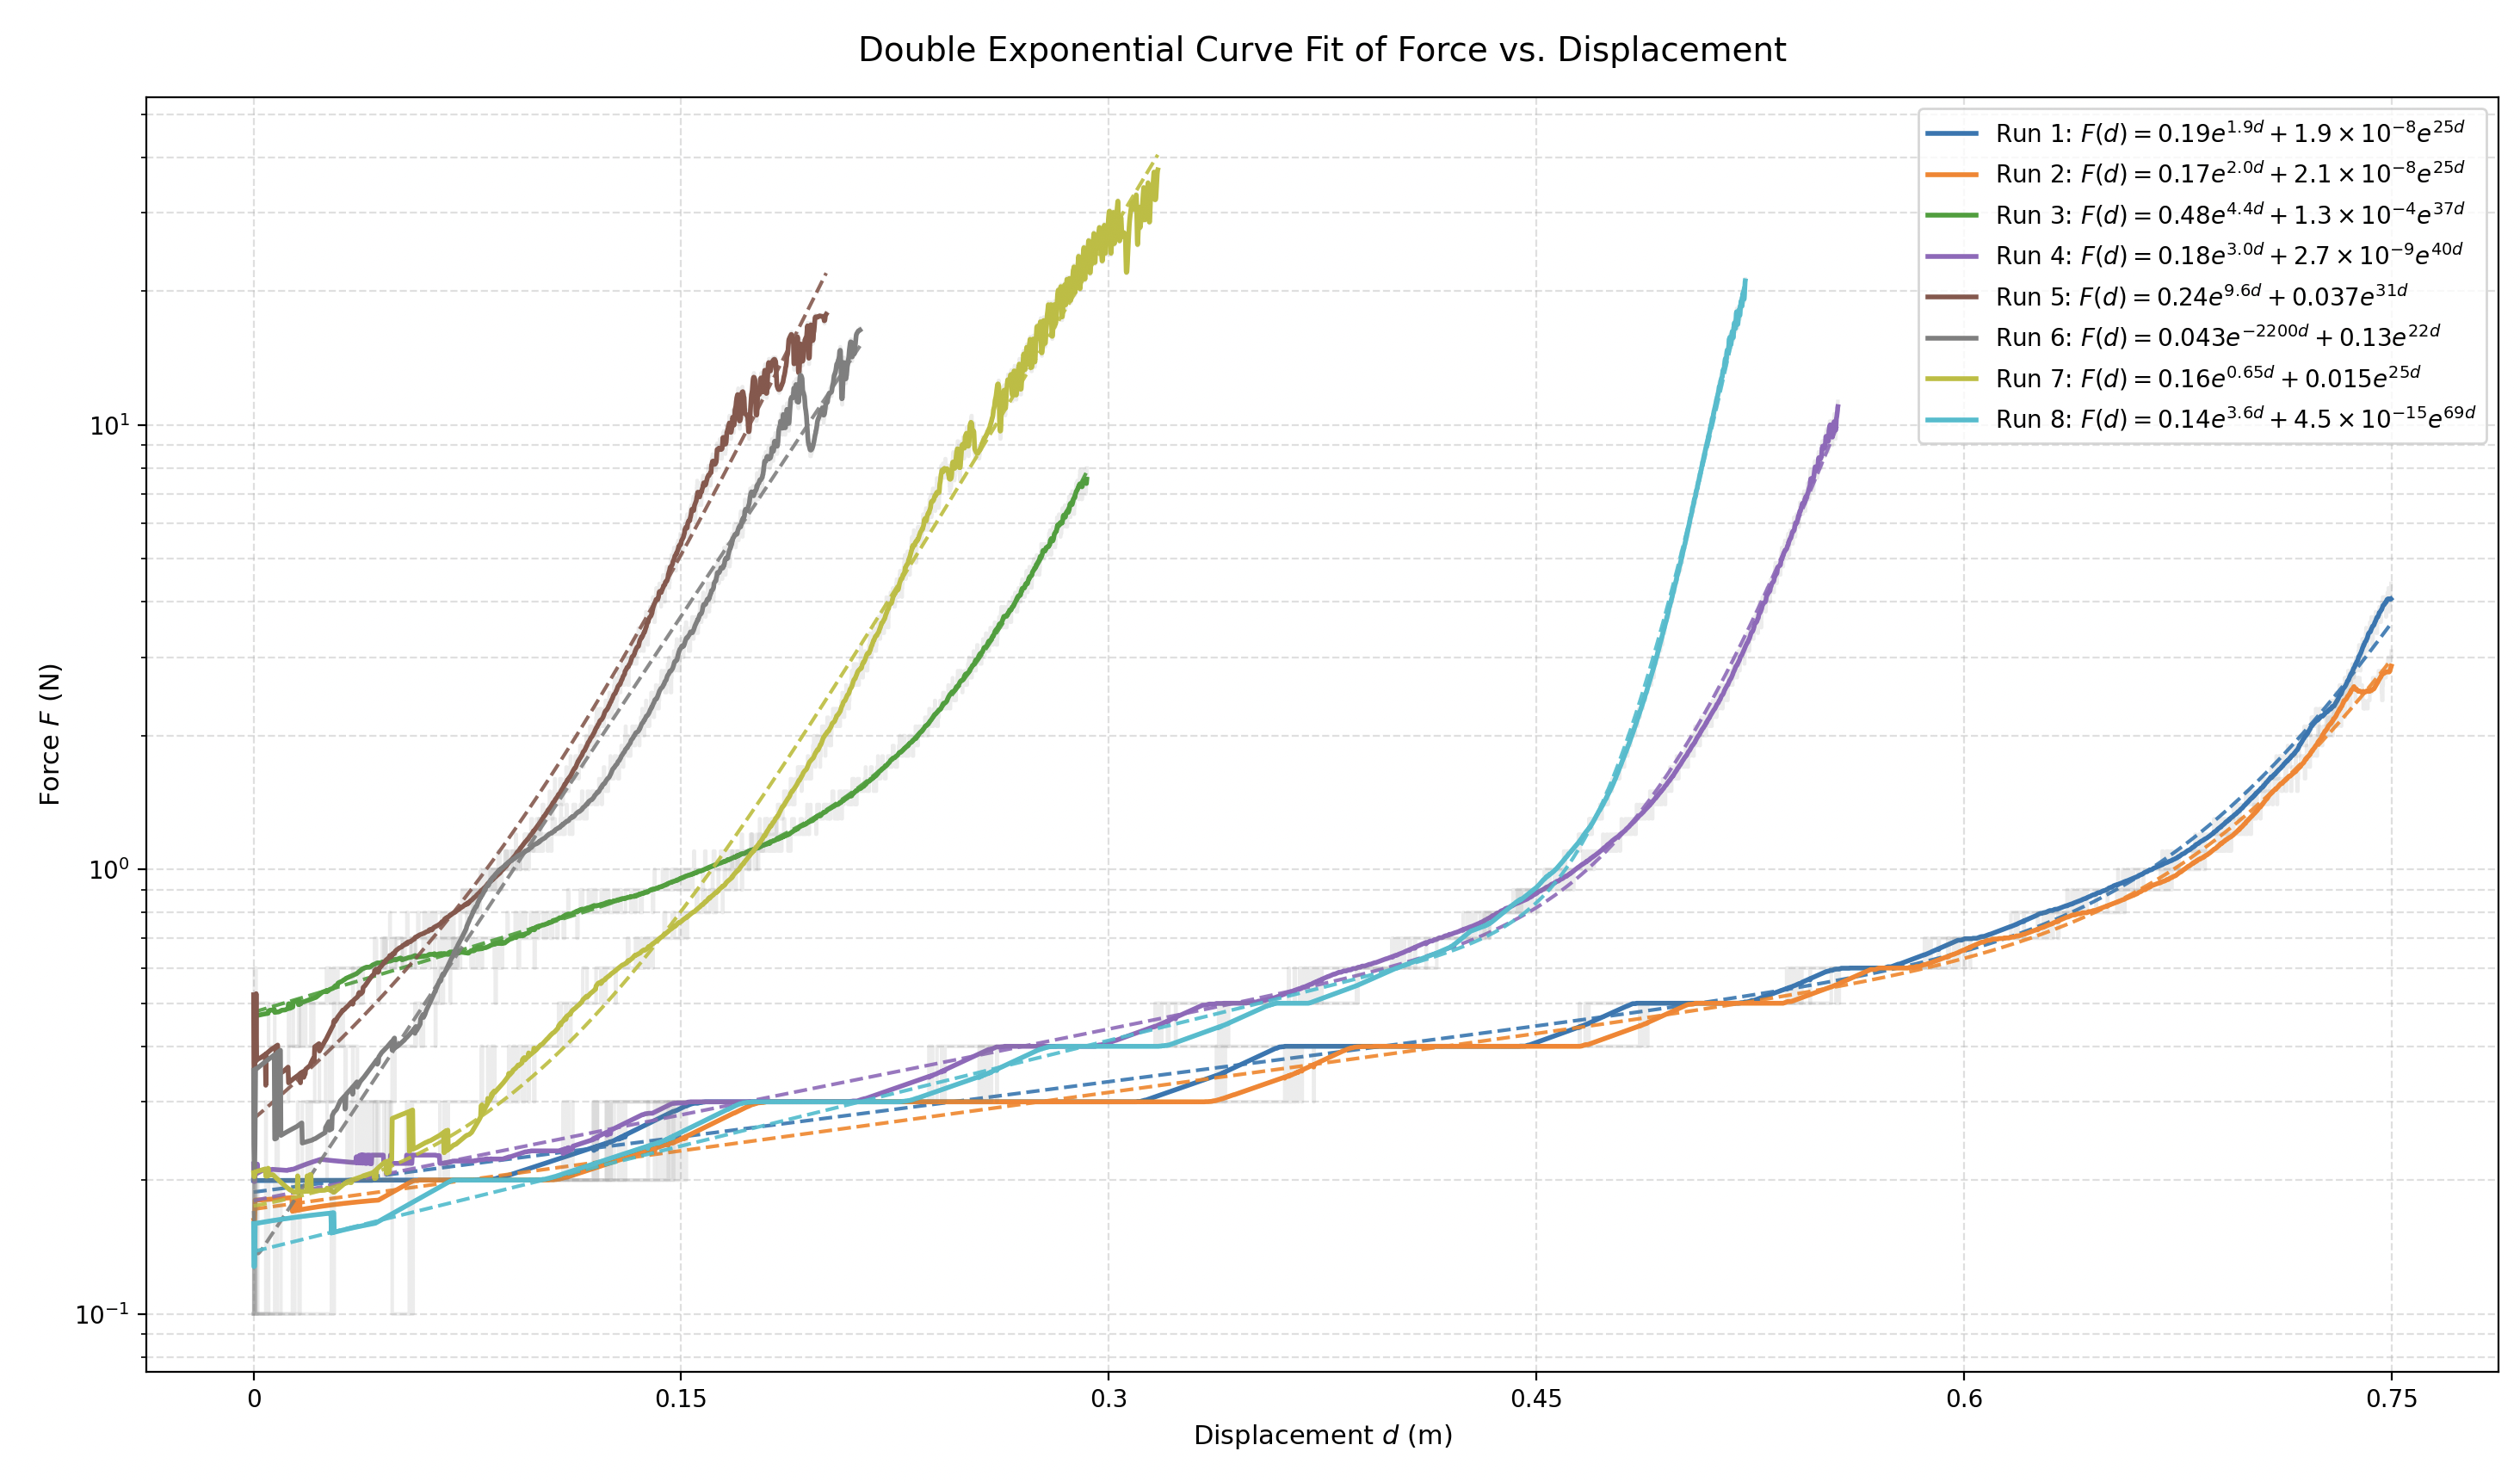
\includegraphics[width=0.7\textwidth]{figs/instron_plot.png}
    \caption{Instron force-displacement data, with raw quantized data (grey), smoothed data (solid colored), and curve fit (dashed colored).}\label{fig:yoyo}
\end{figure}

\end{document}
